\documentclass{article}
\usepackage{tikz,amsmath}
\usetikzlibrary{positioning}
\title{\vspace{-4cm}MATH 222 Assignment Three}
\author{Oliver Tonnesen\\V00885732}
\date{October 17, 2018}
\begin{document}
\maketitle
\renewcommand{\thesubsection}{\thesection.\alph{subsection}}
\section{} % Section 1
\subsection{}
	We consider the 4 women to be a single unit that can be permuted in $4!$ different ways.
	This, in addition to the 6 men, makes up 7 units to arrange, so in total we have
	\[7!4!\]
	such permutations.
\subsection{}
	First we arrange the 6 men in one of $6!$ ways. Then, we count the number of
	4-permutations of the 7 slots between the men in which to put each of the
	4 women.  So we end up with
	\[6!P(7,4)\]
	such permutations.
\subsection{}
	We will count the number of ways in which we can arrange the 10 people such that exactly
	3 women sit together and 1 is alone, and such that all 4 women sit together. We will then
	subtract these two numbers from the total number of ways in which we can arrange the 10
	people, $10!$.
	\newline
	First we arrange the 6 men into one of $6!$ permutations. Then we count the 2-permutations
	of the 7 slots: one for the group of 3, and one for the group of 1. Then we permute the
	group of 3 women. So we have $6!P(7,2)3!$ permutations in which exactly 3 women sit together.
	\newline
	Recall from 1.a that the number of permutations in which exactly 4 women sit together is $7!4!$,
	so overall we have
	\[10!-6!P(7,2)3!-7!4!\]
	such permutations.
\section{} % Section 2
\subsection{}
	First we construct a string of length 8 consisting only of elements of $\{b,c,d\}$.
	Then we have 9 slots in which to place each a, so we have a total of
	\[3^8\cdot9^4\]
	such permutations.
\subsection{}
	We construct the string similarly to above, but we place the 5 b's after the 4 a's.
	So we construct a string of length 3 consisting only of elements of $\{c,d\}$.
	Then we have 4 slots for each of the 4 a's, and after this we have 8 slots for each
	of the 5 b's:
	\[2^3\cdot4^4\cdot8^5\]
\subsection{}
	Note that this problem is isomorphic to counting the number of binary strings of length
	15 containing 3 1's and 12 0's. Each 0 represents a single character in lexicographical
	order, with 1's segmenting the types of character. So in total, we have
	\[15\choose3\]
	such permutations.
\section{} % Section 3
\subsection{}
	The number of ways we can press a pair of buttons is $5\choose2$, so in addition to the
	5 individual buttons, there are $5+{5\choose2}=15$ distinct possible actions. Three of
	these actions in a row thus allows for
	\[15^3\]
	possible sequences of actions.
\subsection{}
	This problem is easily solved using a decision tree. On each branch, we will count the
	number of digits in our action (1 or 2) and each vertex will represent the number of
	choices we have left:
	\newline
	\newline
	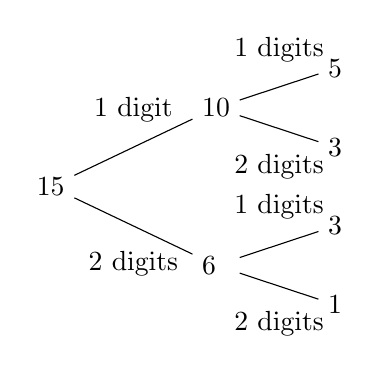
\begin{tikzpicture}
		\node												(0)		{15};
		\node[node distance=15mm,right=of 0,yshift=10mm]	(1)		{10};
		\node[node distance=15mm,right=of 0,yshift=-10mm]	(2)		{6\hphantom{0}};
		\node[distance=15mm,right=of 1,yshift=5mm]			(11)	{5};
		\node[distance=15mm,right=of 1,yshift=-5mm]			(12)	{3};
		\node[distance=15mm,right=of 2,yshift=5mm]			(21)	{3};
		\node[distance=15mm,right=of 2,yshift=-5mm]			(22)	{1};

		\draw	(0)	--	(1)		node[midway,above=2mm] {1 digit};
		\draw	(0)	--	(2)		node[midway,below=2mm] {2 digits};
		\draw	(1)	--	(11)	node[midway,above=2mm] {1 digits};
		\draw	(1)	--	(12)	node[midway,below=2mm] {2 digits};
		\draw	(2)	--	(21)	node[midway,above=2mm] {1 digits};
		\draw	(2)	--	(22)	node[midway,below=2mm] {2 digits};
	\end{tikzpicture}
	\newline
	\newline
	So if we add up all the path from the root to each leaf, we'll get the number of possible
	sequences of actions:
	\[15(10(5+3)+6(3+1))\]
\section{} % Section 4
\subsection*{Algebraic}
	\begin{align*}
		{n\choose{k}}{k\choose{r}}&=\frac{n!}{k!(n-k)!}\frac{k!}{r!(k-r)!}\\
		&=\frac{n!}{k!(n-k)!}\frac{k!}{r!(k-r)!}\frac{(n-r)!}{(n-r)!}\\
		&=\frac{n!}{r!(n-r)!}\frac{k!(n-r)!}{k!(k-r)!(n-k)!}\\
		&={n\choose{r}}\frac{k!(n-r)!}{k!(k-r)!(n-k)!}\\
		&={n\choose{r}}\frac{(n-r)!}{(k-r)!(n-k)!}\\
		&={n\choose{r}}\frac{(n-r)!}{(k-r)!(n-k+r-r)!}\\
		&={n\choose{r}}\frac{(n-r)!}{(k-r)!(n-r-k+r)!}\\
		&={n\choose{r}}\frac{(n-r)!}{(k-r)!((n-r)-(k-r))!}\\
		&={n\choose{r}}{{n-r}\choose{k-r}}\\
	\end{align*}
\subsection*{Combinatorial}
	Count the number of teams with $k$ people, $r$ of whom are also captains, out of $n$ people.
	\newline
	\newline
	Method 1: Select $k$ people out of $n$: $n\choose{k}$, then select $r$ captains out of $k$:
	$k\choose{r}$. There are ${n\choose{k}}{k\choose{r}}$ ways to choose such a team.
	\newline
	\newline
	Method 2: Select r captains out of $n$ people: $n\choose{r}$, then select the rest of the
	team that will not be captains: ${{n-r}\choose{k-r}}$. There are ${n\choose{r}}{{n-r}\choose{k-r}}$
	ways to choose such a team.
	\newline
	\newline
	So, since these two methods both count the same thing,
	${n\choose{k}}{k\choose{r}}={n\choose{r}}{{n-r}\choose{k-r}}$.
\section{} % Section 5
\subsection{}
	First disperse the red balls: $20\cdot19\cdot18\cdot17\cdot16=\frac{20!}{15!}$. Then disperse
	the blue balls: $20\cdot19\cdot\ldots\cdot13=\frac{20!}{12!}$
	So the total number is
	\[\frac{20!}{15!}\cdot\frac{20!}{12!}\]
\subsection{}
	There are two cases: there is one red ball in the first box, or there is no red ball in the
	first box.
	\newline
	\newline
	In the case that there is one red ball in the first box, there are 4 more red balls
	to disperse into the remaining 19 boxes, and 7 blue balls to disperse into the 20 boxes (since
	one blue ball must always be put into the first box). So there are $19^4\cdot20^7$ ways to
	disperse the balls in the first case.
	\newline
	\newline
	In the case that there is no red ball in the first box, there are 5 red balls to disperse into
	the remaining 19 boxes, and, again, 7 blue balls to disperse into the 20 boxes. So there are
	$19^5\cdot20^7$ ways to disperse the balls in this second case.
	\newline
	\newline
	Overall, then, there are
	\[19^4\cdot20^7+19^5\cdot20^7=20^8\cdot19^4\]
	ways to disperse the balls in total.
\section{} % Section 6
	Recall the Multinomial Theorem:\\
	In expansion of $(x_1+x_2+\ldots+x_t)^n$, each term is of the form
	$x_1^{n_1}\cdot{x_2^{n_2}}\cdot\ldots\cdot{x_t^{n_t}}$ and its coefficient is
	$n\choose{n_1,n_2,\ldots,n_t}$.
	\newline
	\newline
	We will use the Multinomial Theorem to solve this problem:
	\[(2w)^3(-5x)^1(7y)^3(z)^5\implies(2)^3(-5)^1(7)^3(1)^5\]
	is the coefficient formed by the coefficients in the original multinomial,
	and the coefficient given by the Multinomial Theorem is
	\[\frac{15!}{3!3!5!1!}=\frac{15!}{3!3!5!}\]
	So the coefficient of $w^3xy^3z^5$ is
	\[\frac{15!}{3!3!5!}\cdot(2)^3(-5)^1(7)^3(1)^5\]
\section{} % Section 7
	Let $O=\{1,3,\ldots,99\}$ and $E=\{2,4,\ldots,100\}$.
	\newline
	\newline
	We will consider two cases: the case where we have 8 even numbers and one odd,
	and the case where we have 8 odd numbers and one even.
	\newline
	\newline
	In the case we have 8 even numbers and one odd, we will first choose the odd.
	Now there are two sub-cases: the case where we choose 1, and the case where we do not choose 1.
	In the case we chose 1, we must choose 2 as one of our even numbers to satisfy the condition that
	there is a pair of consecutive numbers. We now choose 7 more numbers from $E\setminus\{2\}$:
	${|E|-1}\choose7$. Overall for this case there are $49\choose7$ ways to choose.
	In the case we did not choose 1, we chose one odd number from $O\setminus\{1\}$:
	${{|O|-1}\choose1}={49\choose1}=49$. We must choose the even number either before or after our odd
	number: 2 ways. We then must choose 7 more even numbers from $E\setminus\{$our chosen odd number $\pm1\}$:
	${{|E|-2}\choose7}={48\choose7}$.
	\newline
	\newline
	So overall for the case where we have 8 even numbers and one odd, there are
	\[{49\choose7}+49\cdot2\cdot{48\choose7}\]
	ways of choosing.
	\newline
	\newline
	Notice that the exact same logic can be applied to the case where we have 8 odd numbers and one even,
	except two sub-cases are the case where we choose 100 and the case where we do not choose 100 as our
	one even number.
	\newline
	\newline
	So overall, the total number of ways in which we can select 9 distinct numbers from the set
	$\{1,2,\ldots,100\}$ that contain exactly one pair of consectutive numbers is
	\[2\Bigg({49\choose7}+49\cdot2\cdot{49\choose7}\Bigg)\]
\end{document}
